%#vertical 24
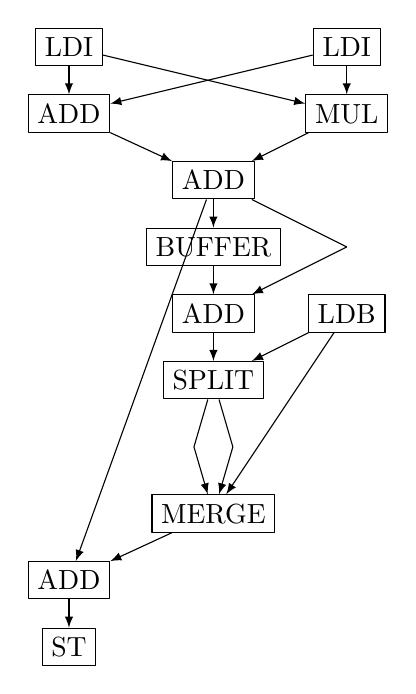
\begin{tikzpicture}[>=latex,line join=bevel,]
%%
\node (ldb) at (200bp,130bp) [draw=black,rectangle] {LDB};
  \node (h_st) at (100bp,10bp) [draw=black,rectangle] {ST};
  \node (add4) at (100bp,34bp) [draw=black,rectangle] {ADD};
  \node (add3) at (152bp,130bp) [draw=black,rectangle] {ADD};
  \node (add2) at (152bp,178bp) [draw=black,rectangle] {ADD};
  \node (add1) at (100bp,202bp) [draw=black,rectangle] {ADD};
  \node (ldi2) at (200bp,226bp) [draw=black,rectangle] {LDI};
  \node (ldi1) at (100bp,226bp) [draw=black,rectangle] {LDI};
  \node (merge) at (152bp,58bp) [draw=black,rectangle] {MERGE};
  \node (split) at (152bp,106bp) [draw=black,rectangle] {SPLIT};
  \coordinate (aux) at (200bp,154bp);
  \node (mul1) at (200bp,202bp) [draw=black,rectangle] {MUL};
  \node (buff) at (152bp,154bp) [draw=black,rectangle] {BUFFER};
  \draw [->,solid] (ldi2) -- (add1);
  \draw [->,solid] (add4) -- (h_st);
  \draw [->,solid] (add2) -- (buff);
  \draw [->,solid] (aux) -- (add3);
  \draw [->,solid] (ldb) -- (split);
  \draw [->,solid] (buff) -- (add3);
  \draw [->,solid] (ldb) -- (merge);
  \draw [->,solid] (ldi2) -- (mul1);
  \draw [->,solid] (ldi1) -- (mul1);
  \draw [solid] (add2) -- (aux);
  \draw [->,solid] (merge) -- (add4);
  \draw [->,solid] (mul1) -- (add2);
  \draw [->,solid] (add3) -- (split);
  \draw [->,solid] (split) -- (145bp,82bp) -- (merge);
  \draw [->,solid] (split) -- (159bp,82bp) -- (merge);
  \draw [->,solid] (ldi1) -- (add1);
  \draw [->,solid] (add1) -- (add2);
  \draw [->,solid] (add2) -- (add4);
%
\end{tikzpicture}

